\documentclass[12pt,letterpaper]{report}


\usepackage[utf8]{inputenc}
\usepackage[spanish]{babel}
\usepackage[table]{xcolor}
\usepackage{xcolor}
\usepackage{fancyhdr}
\usepackage{graphicx}
\usepackage{adjustbox}


\definecolor{royalblue}{HTML}{5B9BD5}
\definecolor{white}{RGB}{0,0,0}

\newcommand{\rowb}{\rowcolor{royalblue}}
\newcommand{\cwhite}{\color{white}}
\newcommand{\mb}{\vspace{0.5cm}}


\pagestyle{myheadings}
\pagestyle{fancy}
\fancyhf{}
%\setlength{\headheight}{10pt}
\renewcommand{\headrulewidth}{2pt}
\renewcommand{\footrulewidth}{1pt}
\fancyhead[L]{Requerimientos}
\fancyhead[C]{}
\fancyhead[R]{Ing. Software 1}
\fancyfoot[L]{19 de febrero de 2019}
%\fancyfoot[C]{\textcopyright xyz}
\fancyfoot[R]{\thepage}


\begin{document}

\begin{titlepage}
	\centering
	
\includegraphics[width=0.25\textwidth]{img/logo.png}\par\vspace{1cm}
	{\scshape\LARGE Universidad nacional de ingeniería \par}
	\vspace{0.25cm}
	{\scshape\Large Facultad de ciencias y sistemas\par}
	\vspace{2.5cm}
	{\large\bfseries Sistema de Investigación, Desarrollo e Innovación (IDI)\\ para el CNU\par}
	\vspace{2cm}

	\vfill
	\begin{center}
		{\Large\itshape Integrantes\par}\vspace{0.5cm}
		Josué David Reyes Molina\\ \vspace{0.15cm}
		Juan Ramón Moreno López\\ \vspace{0.15cm}
		Amy de los Ángeles Rodríguez Gonzalez\\ \vspace{0.15cm}
		Jimmy Geovanny Marcia Galindo\\ \vspace{0.15cm}
		Harold Benito Espinoza Trujillo\\ \vspace{0.15cm}
	\end{center}
	\vfill

% Bottom of the page
	{\large 19 de febrero de 2019\par}
\end{titlepage}

El Consejo Nacional de Universidades (CNU) de Nicaragua es la institución rectora del sistema educativo superior de Nicaragua. Tiene como una de sus finalidades la generación y difusión de conocimientos a través de la investigación, la extensión y la innovación con calidad, pertinencia e interculturalidad; a partir de lo mencionado anteriormente, el CNU, por medio del \textbf{\emph{Sistema de Investigación, Desarrollo e innovación(IDi)}} pretende automatizar el seguimiento y control de la información concerniente a las investigaciones realizadas por las diferentes universidades miembros de esta institución.

Para ello, se presentan los siguientes requerimientos que debe satisfacer el sistema:

\begin{itemize}
\item[1]{
Inicialmente se requiere la \textbf{conceptualización de la investigación}, donde cada universidad presentará a la institución su concepto de investigación como función sustantiva así como las diferentes políticas, normativas y líneas de investigación que poseen.
}


\item[2]{
\textbf{Financiamiento de la Investigación}, se archivará la fuente del financiamiento de las investigaciones, para ello se necesitará el nombre de la fuente, la cantidad de dinero que se programo, lo que se utilizo(Ejecutado) y un porcentaje estimado de la utilización, así como reflejar el total general de cada una de las fuentes que financio el proyecto. Véase la tabla a continuación para más información.

\mb
\centering
	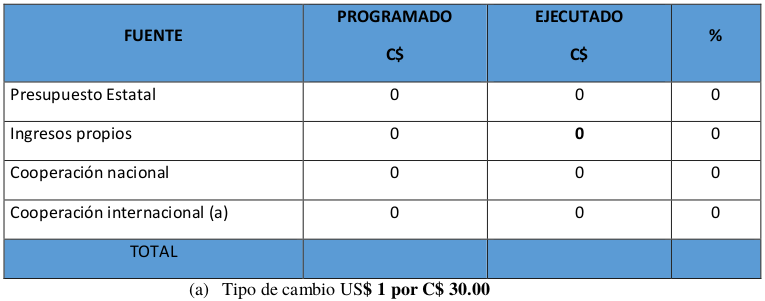
\includegraphics[width=\textwidth]{img/tabla2.png}\par
\mb 
}


\item[3]{
\textbf{Capacidad instalada para la Investigación} (Se reportará trimestral y anual), en esta sección se debe registrar las unidades académicas que se especificarán mediante los siguientes datos: tipo de unidad académica, nombre de la unidad, la ubicación de la unidad y una breve descripción. Cada unidad llevará un número total de capacidad instala, ya que trimestral y anualmente se reportará el total de dicha capacidad instalada, de cada una. Dicha información tiene la siguiente estructura:
}
\textbf{
\begin{center}
\begin{tabular}{|l|c|}
	\hline
	\rowb \cwhite Unidad académica & \cwhite Total\\ \hline
	Centros de investigación & 0\\ \hline
	Unidad de investigación & 0\\ \hline
	Grupos de investigación & 0\\ \hline
	Laboratorios centrales especializados & 0\\ \hline
	Laboratorios especializados & 0\\ \hline
	Programas y proyectos especiales & 0\\ \hline
	Talleres & 0\\ \hline
	Estaciones y fincas experimentales & 0\\ \hline
	Granjas especializadas & 0\\ \hline
	Unidades Especializadas & 0\\ \hline
	Vicerrectoría de Investigación, Posgrado y Proyección Social & 1\\ \hline
	Dirección de Investigación & 1\\ \hline
	Comisión de investigación de recinto & 0\\ \hline
	Coordinación de Investigación por Recinto / Facultad & 1\\ \hline
	Consejo de investigación (Comisión) & 1\\ \hline
	Oficina de relaciones con el entorno & 0\\ \hline
\end{tabular}
\\ \mb
\begin{tabular}{|>{\columncolor{royalblue}}l |l|}
	\hline
	\cwhite Tipo de Unidad Académica: & \\ \hline
	\cwhite Nombre de la Unidad: & Coordinación I+D+i\\ \hline
	\cwhite Ubicación: & Facultad de Ciencias y Sistemas\\ \hline
	\cwhite Descripción: & \\ \hline
\end{tabular}
\end{center}
}

\mb
\item[4]{
\textbf{Total de Horas por profesores de Planta, asignado a la Investigación}, se debe de asignar un profesor de planta a cada investigación y registrar la facultad en la que pertenece dicho profesor, registrar el total de horas por tutorías de monografías, el total de horas por proyecto de investigación y el total de horas en cursos de posgrado.

\mb
\centering
	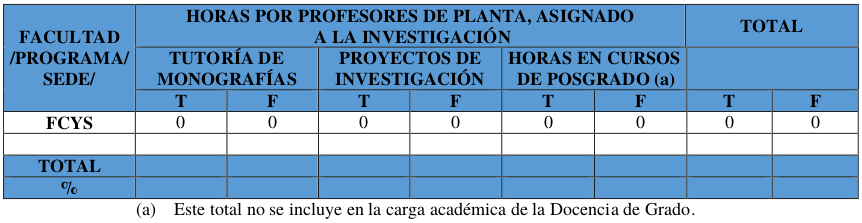
\includegraphics[width=\textwidth]{img/tabla4.png}\par
\mb
}


\item[5]{}


\item[6]{
\textbf{Investigadores de planta (permanentes y contratados) por nivel de formación:}

\begin{itemize}
\item[a]{
\textbf{Investigadores de Planta por nivel de formación}, se clasificará el nivel académico de los investigadores de plantas por facultad, registrará la especialidad de cada uno de ellos (Técnico superior, Licenciatura, maestría, especialidad Médica, Doctorado); así mismo la facultad en la que pertenece.

\mb
\centering
	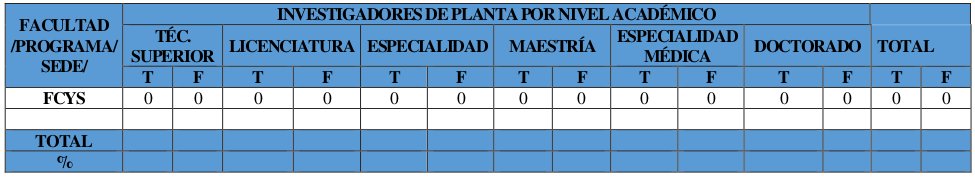
\includegraphics[width=\textwidth]{img/tabla6_1.png}\par
\mb
}


\item[b]{
\textbf{Investigadores contratados por nivel de formación}, se clasificará el nivel académico de los investigadores de contratos determinado por facultad, registrará la especialidad de cada uno de ellos (Técnico superior, Licenciatura, maestría, especialidad Médica, Doctorado); así mismo la facultad en la que pertenece.

\mb
\centering
	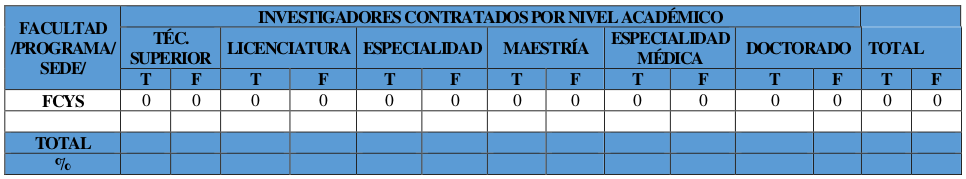
\includegraphics[width=\textwidth]{img/tabla6_2.png}\par
\mb
}

\end{itemize}
}


\item[7]{
\textbf{Investigaciones realizadas por investigadores de planta y docentes – investigadores}, todas las investigaciones son realizadas por investigadores y docentes de investigadores de la planta. Deberá llevar un formato en el cual se especifique de quien son las investigaciones realizadas separando por investigadores de planta y docentes, incluyendo en la tabla el numero de investigaciones y el sexo del investigador. Las investigaciones realizadas deberán llevar control del numero de proyectos en ejecución y los proyectos concluidos ya sean de un investigador de planta o de un docente.

\mb
\centering
	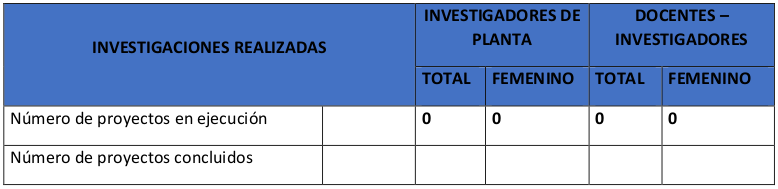
\includegraphics[width=\textwidth]{img/tabla7.png}\par
\mb
}


\item[8]{
\textbf{Tesis de Posgrado}, se registrarán las tesis de posgrado según el numero de tesis en ejecución y tesis concluidas, incluyendo a tutores y estudiantes involucrados. En la tabla se mostrará el número de estudiantes o tutores participantes, así como su sexo.

\mb
\centering
	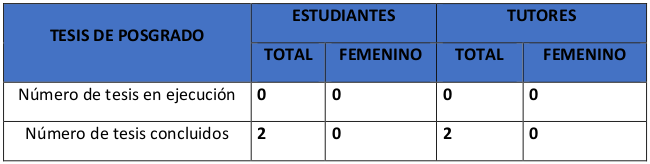
\includegraphics[width=\textwidth]{img/tabla8.png}\par
\mb
}


\item[9]{
\textbf{Investigaciones realizadas por académicos y estudiantes de Posgrado}, las investigaciones de posgrado deberán ser realizadas por académicos y estudiantes de posgrados. Se deberán presentar la cantidad de investigaciones realizadas ya sean en ejecución o terminadas. Se deberá mostrar si las investigaciones que se realizan pertenecen a docentes o estudiantes y mostrar un control de investigaciones realizadas junto con el sexo del autor.

\mb
\centering
	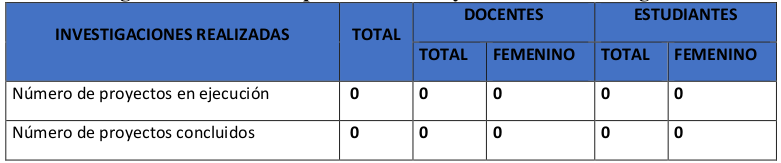
\includegraphics[width=\textwidth]{img/tabla9.png}\par
\mb
}


\item[10]{
\textbf{Trabajos presentados en eventos científicos nacionales e internacionales}, En los eventos, se pueden presentar trabajos científicos tanto nacionales como internacionales. Estos trabajos tienen los siguientes atributos: nombre del trabajo, nombres de los investigadores y el evento en el cual se esta presentando. Para más información se muestra la siguiente tabla.

\mb
\centering
	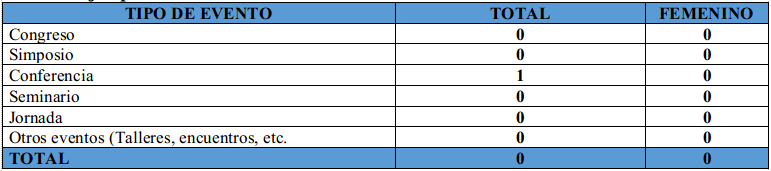
\includegraphics[width=\textwidth]{img/tabla10.png}\par
\mb 
}


\item[11]{
\textbf{Eventos científicos organizados por las universidades}, se puede realizar varios eventos científicos a lo largo del año. Los eventos están clasificados por el Tipo de evento, ademas se guarda la fecha de realización, lugar de realización y una breve descripción del evento. Los eventos pueden ser organizados por cualquiera de la universidades autorizadas por el CNU, por el mismo CNU o por otras instituciones. En los eventos se debe registrar a todos los participantes, tanto a docentes, estudiantes y otros participantes. En este registro se debe almacenar el sexo de los participantes.
}


\item[12]{
\textbf{Participación en eventos científicos organizados por el CNU y otras instituciones}, el sistema deberá realizar reportes acerca de los eventos, como la cantidad de participantes en un evento desagregado por su clasificación y sexo. También deberá mostrar tanto datos generales como las fecha y lugar de realización y datos mas específicos como los trabajos que se presentaron en cada evento, los autores de cada trabajo desagregados por el tipo de evento. La siguiente tabla puede apreciarse más informcación, tanto para este punto como para el anterior.

\mb
\centering
	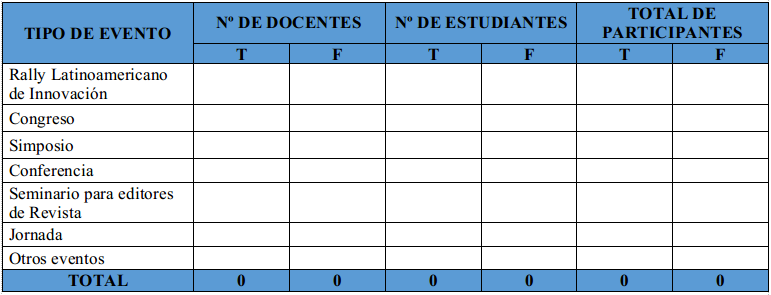
\includegraphics[width=\textwidth]{img/tabla11_12.png}\par
\mb 
}


\item[13]{
\textbf{Publicaciones}, se requiere presentar el listado de los trabajos publicados. Se sugiere que dicho listado sea elaborado a modo de referencia bibliográfica utilizando el estilo de las normas APA, indicando el nombre de los autores de la publicación. El listado debe mostrar el nombre de la publicación, el tipo de publicación, la fecha y los autores.
}


\item[14]{
\textbf{Diplomados y Cursos Libres (como actividades del trabajo de Investigación)}, debe mostrarse el listado de los diplomados y cursos libres, el listado debe contener el nombre del diplomado/curso, así como la cantidad de mujeres matriculadas dentro de cada uno.
}


\item[15]{
\textbf{Investigaciones realizadas por los estudiantes de grado}, se requiere presentarun listado de los trabajos realizados, dicho listado debe estar compuesto por el nombre de la investigación, el nombre de los autores, el nombre de los(as) tutores y el tipo de jornada científica en la que es presentada la investigación. Los resultados deben estar acompañados por el número total de autores así como el número total de autoras femeninas, de igual manera presentar el número total de tutores y tutoras femeninas. Para más información se muestra la siguiente tabla.

\mb
\centering
	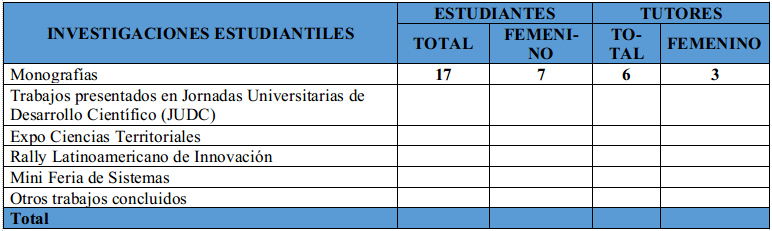
\includegraphics[width=\textwidth]{img/tabla15.png}\par
\mb 
}


\item[16]{
\textbf{Resumen de Indicadores relacionados con el trabajo de Investigación}, se necesita obtener en resumen los indicadores de los diferentes trabajos de investigación junto con el número total de investigaciones que pertenecen a ese tipo.
}


\item[17]{
\textbf{Valoración cualitativa global de la Investigación en el año}, es necesario mostrar un informe de los resultados obtenidos a lo largo del período en que se muestren los diferentes logros realizados, las diferentes dificultades, actividades de impacto en la función Investigación y las perspectivas para el siguiente período.
}
\end{itemize}

\end{document}